\chapter{Evaluation}\label{ch:evaluation}
In this chapter, the individual algorithms, as well as the final performance of the combined system, will be evaluated.
First, the depth from motion algorithm will be evaluated based on different materials and their resulting confidence maps in section~\ref{sec:eval-depth-from-motion}.
Section~\ref{sec:point-clouds} will then evaluate the two point cloud datastructures as described in section~\ref{subsec:inserting-new-points-into-the-point-cloud}.
In section~\ref{sec:eval-ransac-algorithm}, the RANSAC algorithm will be evaluated based on synthetic data, as well as real world data.
Finally, in section~\ref{subsec:application-performance-full-room}, the application performance will be evaluated on the use case of a full room scan.
CloudCompare~\cite{daniel_girardeau-montaut_cloudcompare_nodate}, an open-source tool for working with 3D point clouds, will be used for the evaluation of the point clouds and the RANSAC algorithm.
%klare begründung => Anforderung erfüllt ja oder nein

\section{Depth from Motion}\label{sec:eval-depth-from-motion}
As the depth from motion algorithm greatly differs in its performance based on the amount of texture in the captured scene~\cite{google_llc_arcore_doc},
this section will evaluate different materials based on their resulting confidence maps, as retrieved from the ARCore Raw Depth API\@.
In figure~\ref{fig:materials}, the confidence maps of different materials are shown - the camera image on top, the confidence map on the bottom.

\begin{figure}[h!tb]
    \centering
    % First row
    \begin{subfigure}[b]{0.25\textwidth}
        \centering
        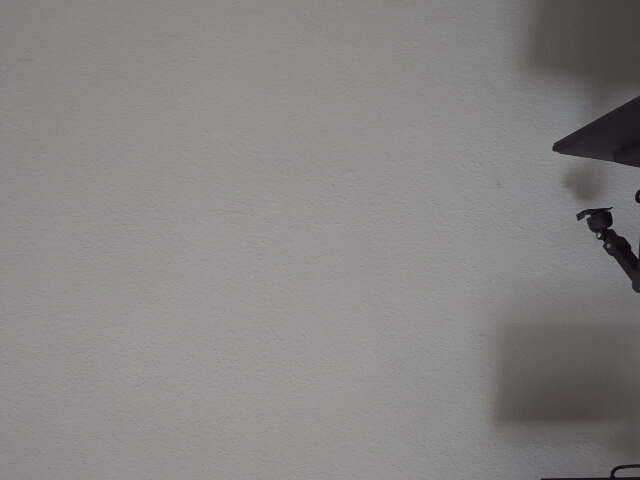
\includegraphics[width=0.9\linewidth]{images/materials/wall-far-cam}
    \end{subfigure}%
    \begin{subfigure}[b]{0.25\textwidth}
        \centering
        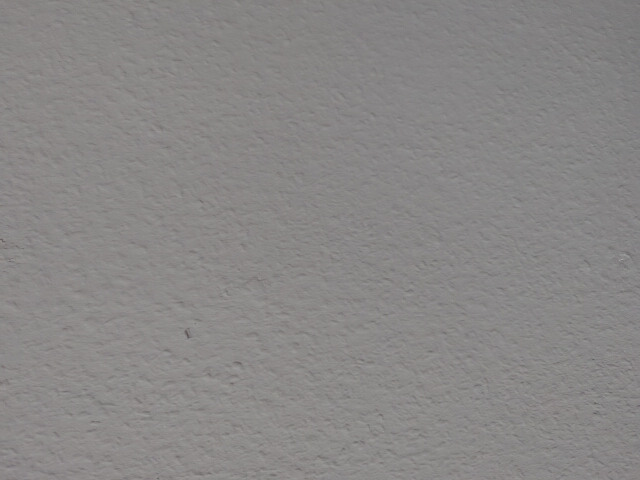
\includegraphics[width=0.9\linewidth]{images/materials/wall-close-cam}
    \end{subfigure}%
    \begin{subfigure}[b]{0.25\textwidth}
        \centering
        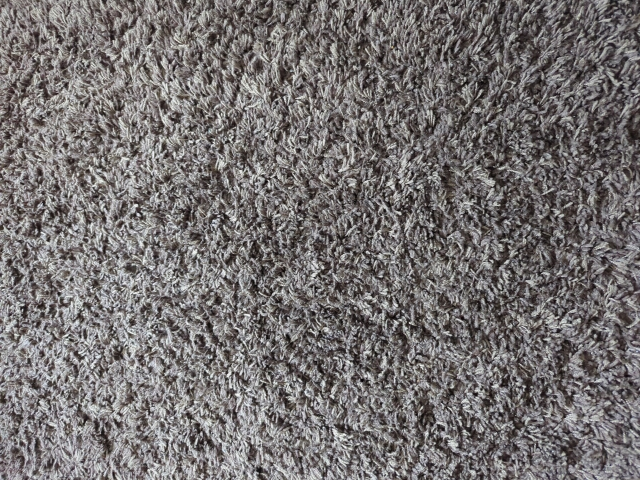
\includegraphics[width=0.9\linewidth]{images/materials/carpet-cam}
    \end{subfigure}%
    \begin{subfigure}[b]{0.25\textwidth}
        \centering
        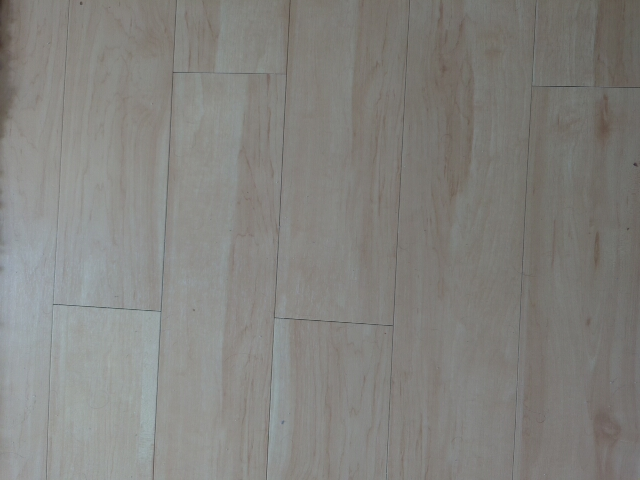
\includegraphics[width=0.9\linewidth]{images/materials/wood-cam}
    \end{subfigure}%

    \begin{subfigure}[b]{0.25\textwidth}
        \centering
        
\includegraphics[width=0.9\linewidth]{images/materials/wall-far-conf}
        \caption{Wall, 1.5m}
        \label{fig:material-wall-far}
    \end{subfigure}%
    \begin{subfigure}[b]{0.25\textwidth}
        \centering
        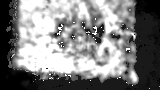
\includegraphics[width=0.9\linewidth]{images/materials/wall-close-conf}
        \caption{Wall, 0.5m}
        \label{fig:material-wall-close}
    \end{subfigure}%
    \begin{subfigure}[b]{0.25\textwidth}
        \centering
        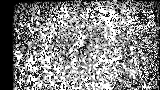
\includegraphics[width=0.9\linewidth]{images/materials/carpet-conf}
        \caption{Carpet}
        \label{fig:material-carpet}
    \end{subfigure}%
    \begin{subfigure}[b]{0.25\textwidth}
        \centering
        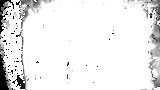
\includegraphics[width=0.9\linewidth]{images/materials/wood-conf}
        \caption{Wooden floor}
        \label{fig:material-wood}
    \end{subfigure}%

    \vspace{0.5em}

    % First row
    \begin{subfigure}[b]{0.25\textwidth}
        \centering
        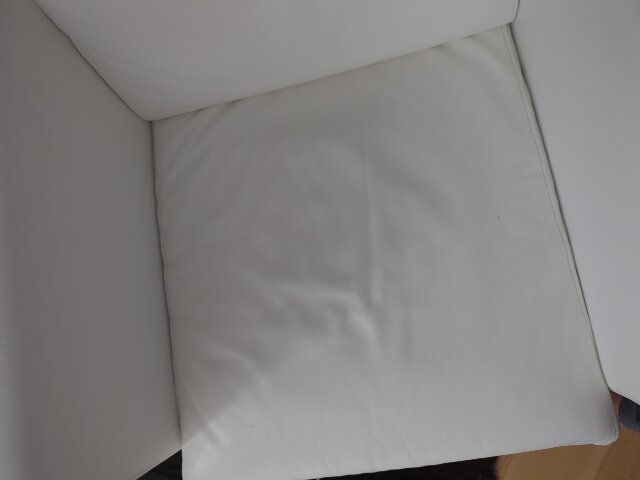
\includegraphics[width=0.9\linewidth]{images/materials/leather-cam}
    \end{subfigure}%
    \begin{subfigure}[b]{0.25\textwidth}
        \centering
        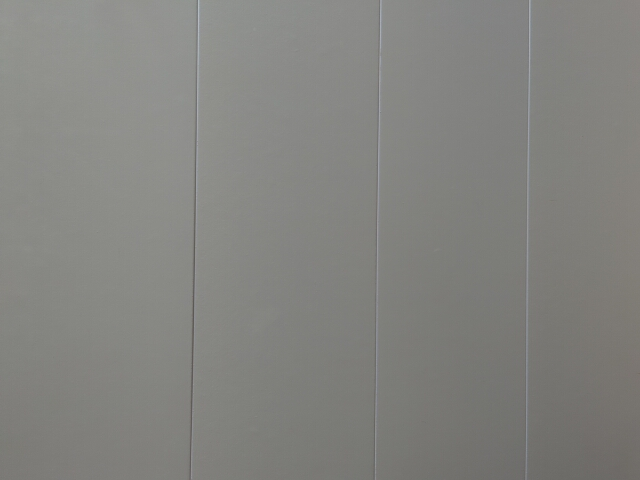
\includegraphics[width=0.9\linewidth]{images/materials/whiteFurniture-cam}
    \end{subfigure}%
    \begin{subfigure}[b]{0.25\textwidth}
        \centering
        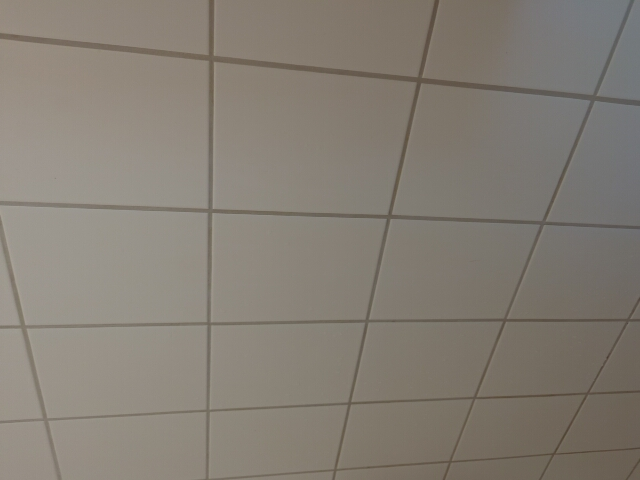
\includegraphics[width=0.9\linewidth]{images/materials/tiles-cam}
    \end{subfigure}%
    \begin{subfigure}[b]{0.25\textwidth}
        \centering
        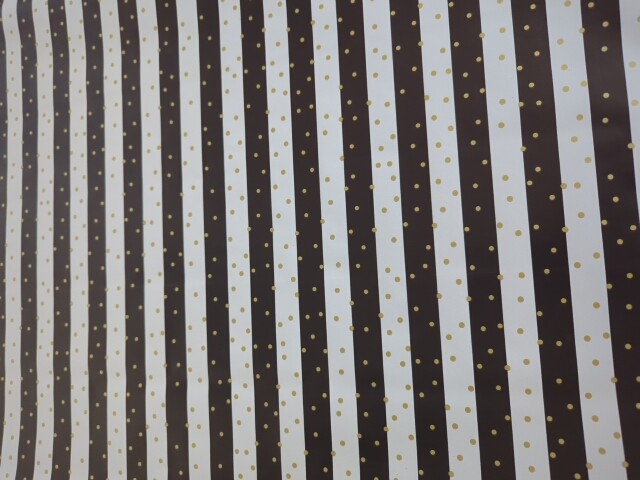
\includegraphics[width=0.9\linewidth]{images/materials/giftpaper-cam}
    \end{subfigure}%

    \begin{subfigure}[b]{0.25\textwidth}
        \centering
        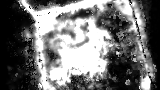
\includegraphics[width=0.9\linewidth]{images/materials/leather-conf}
        \caption{Leather armchair}
        \label{fig:material-leather}
    \end{subfigure}%
    \begin{subfigure}[b]{0.25\textwidth}
        \centering
        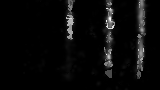
\includegraphics[width=0.9\linewidth]{images/materials/whiteFurniture-conf}
        \caption{White furniture}
        \label{fig:material-whiteFurniture}
    \end{subfigure}%
    \begin{subfigure}[b]{0.25\textwidth}
        \centering
        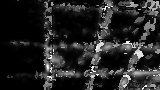
\includegraphics[width=0.9\linewidth]{images/materials/tiles-conf}
        \caption{Bathroom tiles}
        \label{fig:material-tiles}
    \end{subfigure}%
    \begin{subfigure}[b]{0.25\textwidth}
        \centering
        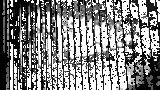
\includegraphics[width=0.9\linewidth]{images/materials/giftpaper-conf}
        \caption{Gift paper}
        \label{fig:material-giftpaper}
    \end{subfigure}%

    \caption{Comparison of confidence maps of different materials. Camera image on top, confidence map on bottom.}
    \label{fig:materials}
\end{figure}

In figure~\ref{fig:material-wall-close} and~\ref{fig:material-wall-far}, the confidence maps of a wall at different distances is shown.
It is apparent that the confidence map of the wall at 1.5m distance is almost completely black, meaning low confidence.
This is due to the lack of any texture on the wall at this distance.
When moving closer to the wall, the structure of the wall becomes more apparent and the confidence increases greatly.

In figure~\ref{fig:material-carpet}, a carpet with a lot of texture is shown, the resulting confidence map has fairly high confidence on average,
but also has dark sports throughout the map.
This could be a result of the repetitive pattern of the carpet.

The highest confidence of all tested materials is achieved on a wooden floor, as shown in figure~\ref{fig:material-wood}.
This can be attributed to the high amount of texture and value variance throughout the wood, while not being repetitive.
The seams between the wooden planks are also clearly visible.

Figure~\ref{fig:material-leather} shows a leather armchair, which has high confidence on the seams of the chair and
creases of the leather, with low confidence in other areas, where the leather is smoother.
A similar pattern is visible on white furniture and bathroom tiles, in figures~\ref{fig:material-whiteFurniture} and~\ref{fig:material-tiles} respectively,
where the white surface has very low confidence, while the seams between the surfaces have increased confidence.
The gift paper shown in figure~\ref{fig:material-giftpaper} shows a similar effect, but less pronounced.
As the surface itself is striped with dots randomly placed throughout, the confidence is higher overall,
but the striped pattern is still visible in the confidence map, as the stripes themselves contain little texture.

These examples show how the amount of texture on a given surface greatly influences the confidence of the depth from motion algorithm, as expected.
The algorithm performs best on surfaces with high texture, while struggling with low texture surfaces.
Small repetitive patterns can also lead to low confidence, as visible in the carpet example.
It is also important to note that the texture captured by the camera is important, not the texture of the material itself.
This can be seen in the first example of the wall: When capturing from afar, the cameras resolution is too low to capture the texture,
but when moving closer to the wall, the texture of the wall becomes more apparent and the confidence increases.
Lighting conditions will also influence the confidence of the algorithm,
as angled light will create shadows that will increase the texture of the surface~\cite{google_llc_arcore_doc} (not shown in the comparison).

\section{Point Clouds}\label{sec:point-clouds}
This section will evaluate the two point cloud datastructures as described in section~\ref{subsec:inserting-new-points-into-the-point-cloud}.
To evaluate the datastructures, the point cloud is transferred from the mobile application to a computer using
a simple HTTP server with a single endpoint, that accepts a file using a POST request and saves it to disk.
The Android application will then stream the point cloud data, serialized as a PLY file, to the server on a push of a button.
A PLY file is a simple file format for storing 3D point cloud data in plain text
and allows for saving custom properties for each vertex, such as the confidence value of the point.
In all the following images of the point clouds, the confidence value is color-coded,
with green being high confidence and red being low confidence.

\begin{lstlisting}[caption=Example PLY file]
ply
format ascii 1.0
element vertex 6
property float x
property float y
property float z
property float confidence
property uchar red
property uchar green
property uchar blue
end_header
0.1851168 -0.77074146 -0.92582846 1.0 0 255 0
-0.061887983 -0.7755803 -0.79551744 1.0 0 255 0
-0.058628604 -0.7638883 -0.7860476 0.80784315 245 10 0
-0.07720285 -0.75610626 -0.80394375 0.81960785 230 25 0
-0.19774273 -0.6645372 -2.5003948 1.0 0 255 0
-0.09499544 -0.028413996 -2.553247 0.99607843 5 250 0
\end{lstlisting}

%\begin{lstlisting}[caption=HTTP server code, language=Python]
%from fastapi import FastAPI
%from starlette.requests import Request
%
%app = FastAPI()
%
%@app.post("/upload")
%async def upload(request: Request):
%    body = await request.body()
%    body_str = body.decode('utf-8')
%    with open("data.ply", "w") as f:
%        f.write(body_str)
%\end{lstlisting}

\begin{figure}[h!tbp]
    \centering
    \begin{subfigure}[b]{0.33\textwidth}
        \centering
        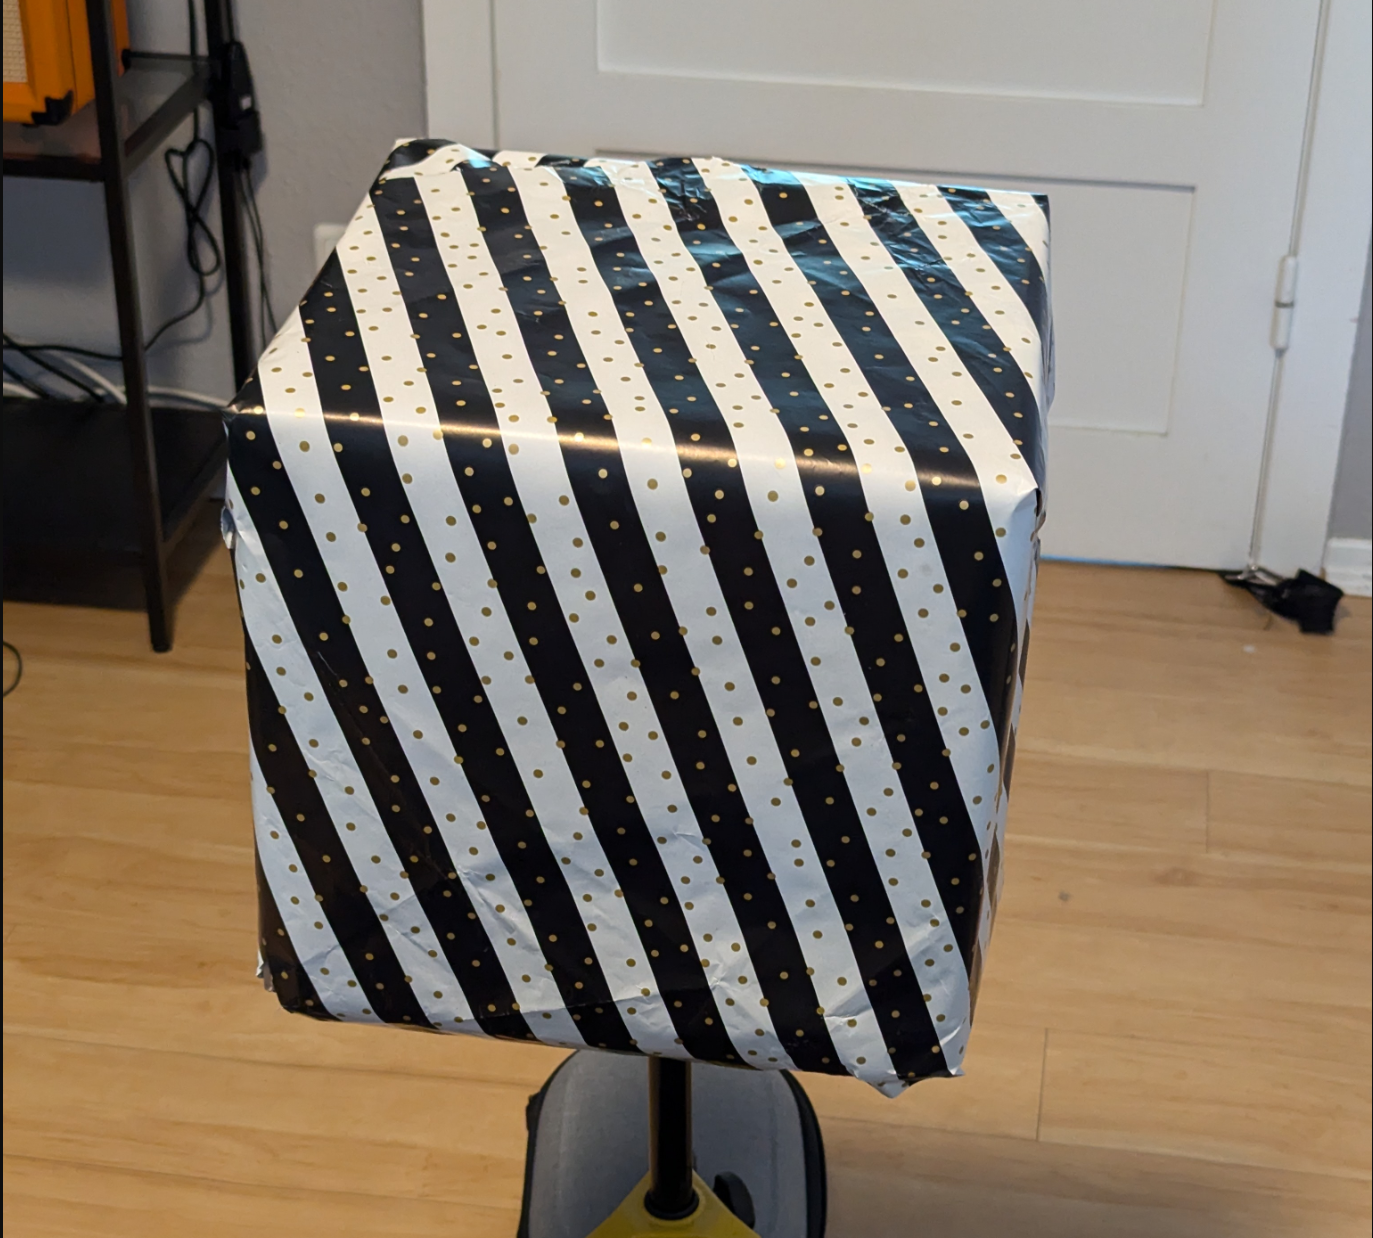
\includegraphics[width=0.9\linewidth]{images/test-setup}
        \caption{Color image of setup}
    \end{subfigure}%
    \begin{subfigure}[b]{0.33\textwidth}
        \centering
        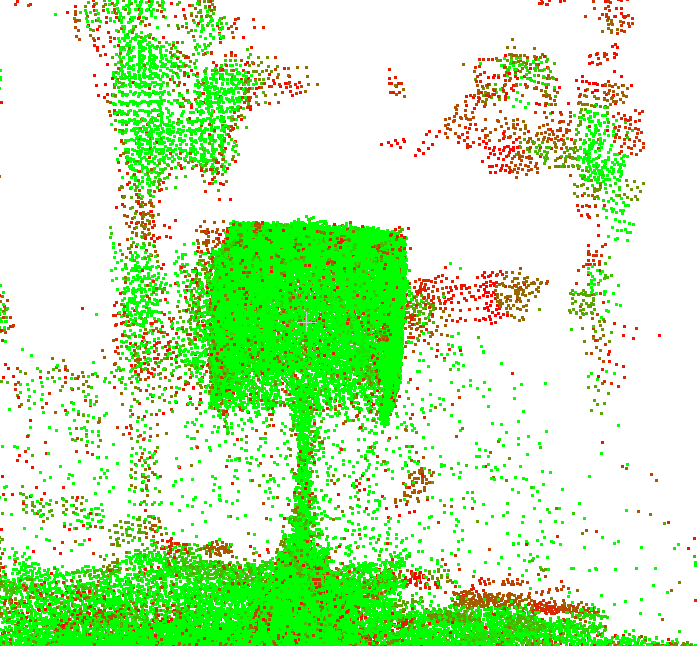
\includegraphics[width=0.9\linewidth]{images/test-setup-cloud}
        \caption{Captured point cloud}
    \end{subfigure}%
    \begin{subfigure}[b]{0.33\textwidth}
        \centering
        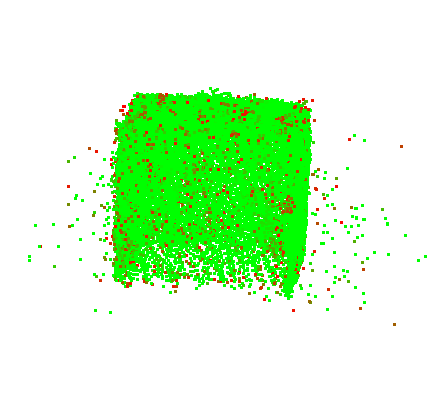
\includegraphics[width=0.9\linewidth]{images/test-setup-segmented}
        \caption{Segmented point cloud}
    \end{subfigure}%
    \caption{Test setup for capturing point clouds}
    \label{fig:test-setup}
\end{figure}

For test data, a cube wrapped with the same gift-paper as in figure~\ref{fig:material-giftpaper} is used, called \textit{test cube} from now on.
The bottom of the test cube is hollow, so in total, 5 faces are visible.
The cube is propped up on stand, to allow for easy segmentation of the point cloud later on,
in order to remove the floor and other objects from the point cloud.
Reproducibility is ensured by using controlled lighting conditions and a fixed setup.
To capture a scan of the test cube, the camera is moved around the cube 3 times, while also moving the camera up and down,
to capture multiple angles for the depth from motion algorithm to work to its full potential.
The full setup is shown in figure~\ref{fig:test-setup}.

\subsection{Quantization Octree vs. Epsilon Octree}\label{subsec:quantization-octree-vs.-epsilon-octree}

A point cloud with a resolution of $s=0.005$m or 5mm is captured for both the quantization octree and the epsilon octree.
In the resulting segmented point cloud, the quantization octree has a total of about 90.000 points,
while the epsilon octree only has about 20.000 points.
This can be explained due to the quantization octree always ending up with the maximal resolution
with enough data added, as it is functionally a three-dimensional grid.
The epsilon octree, on the other hand, will only add points that are within the epsilon threshold of the current point,
which means that gaps between points are at least epsilon wide, but can be wider.
For example, if two points almost 2 epsilon apart, no points will be added between them and the gap will be approximately
2 epsilon wide.
As epsilon is set to $s$, the epsilon octree will have fewer points than the quantization octree with the same resolution.
To compare the two datastructures, the quantization octree will be used with a lower resolution of $s=0.010$m,
which results in a number of points of about 22.000, which is comparable to the epsilon octree at $s=0.005$m.

Figure~\ref{fig:octrees-compairison} shows the raw and segmented point clouds of both datastructures.
From inspecting the raw point cloud visually, it is apparent that the quantization octree has a higher amount of noise.
While the cube is easily recognizable in the point cloud of the epsilon octree, the point cloud of the quantization octree has a lot of noise around the cube.
The quantization octree also has more low-confidence points than the epsilon octree.
This is due to the quantization octree always adding points to the cloud that fall within the threshold,
while the epsilon octree only adds / updates points based on a condition that takes the confidence of the point into account
and ignores lower confidence points that are close to higher confidence points.
As such, the epsilon octree improves the accuracy of the point cloud when new, higher confidence points are added.


\begin{figure}[h!tb]
    \centering
    \begin{subfigure}[b]{0.4\textwidth}
        \centering
        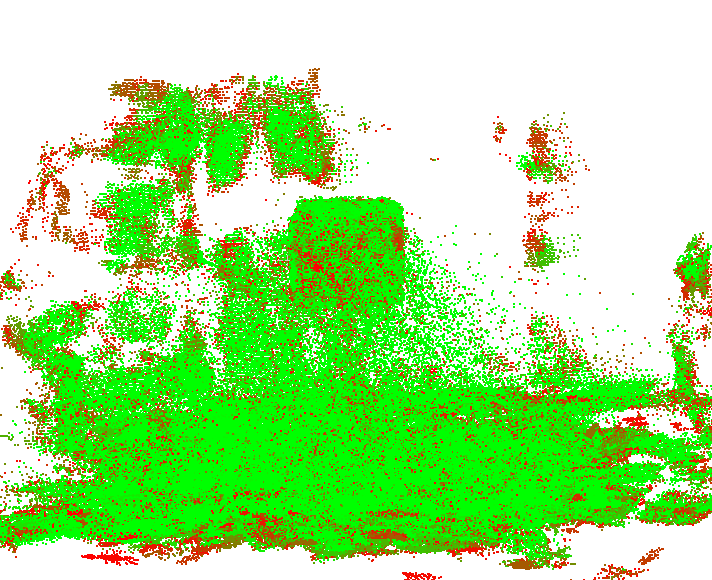
\includegraphics[width=0.9\linewidth]{images/eval-clouds-quant2}
    \end{subfigure}%
    \begin{subfigure}[b]{0.4\textwidth}
        \centering
        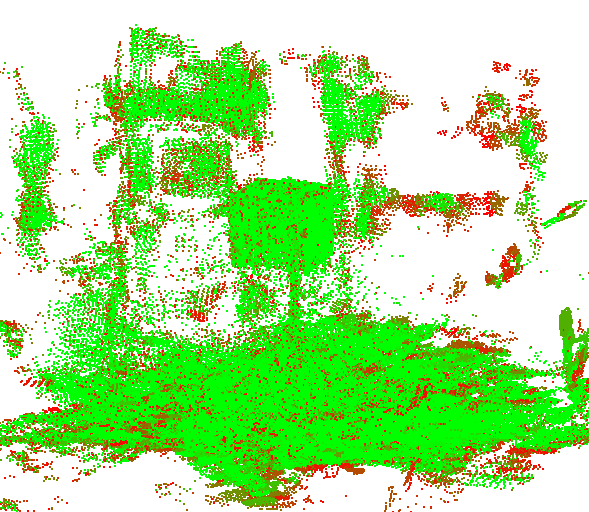
\includegraphics[width=0.9\linewidth]{images/eval-clouds-epsilon}
    \end{subfigure}%

    \begin{subfigure}[b]{0.4\textwidth}
        \centering
        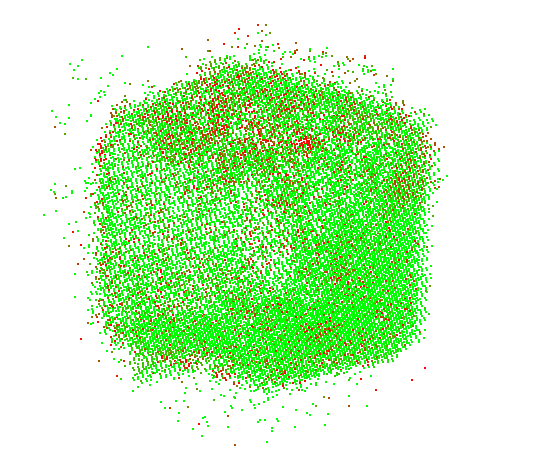
\includegraphics[width=0.9\linewidth]{images/eval-clouds-quant-segmented2}
        \caption{Quantization Octree, $s=0.010$m}
    \end{subfigure}%
    \begin{subfigure}[b]{0.4\textwidth}
        \centering
        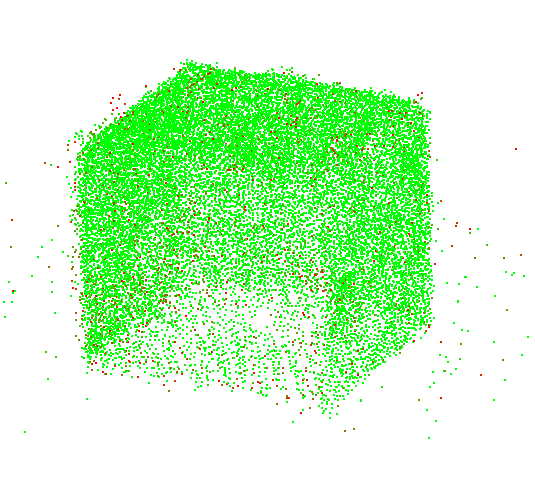
\includegraphics[width=0.9\linewidth]{images/eval-clouds-epsilon-segmented}
        \caption{Epsilon Octree, $s=0.005$m}
        \label{fig:octrees-compairison-epsilon}
    \end{subfigure}%

    \caption{Comparison of Quantization Octree and Epsilon Octree. Raw point cloud on top, segmented on bottom.}
    \label{fig:octrees-compairison}
\end{figure}

To calculate statistics on the point clouds, the real box is measured and a primitive box with matching dimensions is created in CloudCompare.
Using the \textit{fine registration (ICP)} feature, it is possible to align the point clouds to the primitive box.
The underlying algorithm of the fine registration feature is the Iterative Closest Point (ICP) algorithm,
which iteratively minimizes the mean square distance between a "model" shape and a "data" shape~\cite{besl_method_1992}.
Once the point clouds are aligned to the primitive,
the distance between the points of the point cloud and the primitive box can be calculated using the \textit{Cloud/Mesh Distance} feature in CloudCompare.
The result of this calculation can be seen in figure~\ref{fig:octrees-compairison-stats}.
From the histogram, it is apparent that the quantization octree has higher noise than the epsilon octree.
This can also be seen in the standard deviation, which is 0.022 for the quantization octree and 0.011
for the epsilon octree.
This confirms the first suspicion from visual inspection of the point clouds.
The mean distance is also higher for the quantization octree, with 0.0046 compared to 0.0011 for the epsilon octree.
This can be understood as points being 0.5cm and 0.1cm away from the real surface in mean, respectively.
If these points were to be used for primitive detection, this would indicate how far off the detected primitives would be from the real surface.

These results suggest that the epsilon octree is an improvement over the quantization octree in terms of accuracy,
both when it comes to the amount of noise and the distance to the real surface.
As such, the epsilon octree will be used for following evaluations.

\begin{figure}[h!tbp]
    \centering
    \begin{subfigure}[b]{0.5\textwidth}
        \centering
        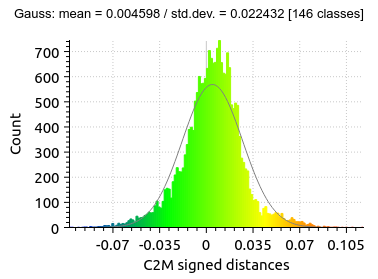
\includegraphics[width=0.9\linewidth]{images/eval-quant-hist}
        \caption{Quantization Octree}
    \end{subfigure}%
    \begin{subfigure}[b]{0.5\textwidth}
        \centering
        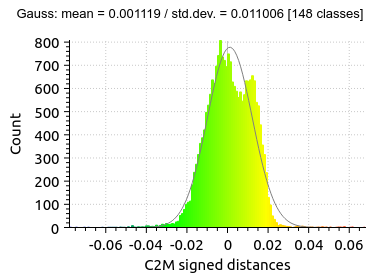
\includegraphics[width=0.9\linewidth]{images/eval-epsilon-hist}
        \caption{Epsilon Octree}
    \end{subfigure}%
    \caption{Histogramm of distances between segmented point cloud points and primitive mesh}
    \label{fig:octrees-compairison-stats}
\end{figure}

\section{RANSAC Algorithm}\label{sec:eval-ransac-algorithm}
In this section, the RANSAC algorithm will be evaluated based on a model of a cube,
first using synthetic data in section~\ref{subsec:tests-on-singular-synthetic-cube} and then using real world data
in section~\ref{subsec:ransac-tests-on-real-world-data}.

\subsection{Tests on Synthetic Cube}\label{subsec:tests-on-singular-synthetic-cube}

A unit cube will be used as a test object to evaluate the RANSAC algorithm.
The cube has been generated with a side length of 1 and a sampling rate of 0.01.
This would equate to a cube with a side length of 1m and a distance of 1cm between points in the real world,
which is comparable to what was used in section~\ref{subsec:quantization-octree-vs.-epsilon-octree}.

\subsubsection{Resilience to Noise}
In figure~\ref{fig:test-noise}, the unit cube is shown with varying noise levels using gaussian noise.
The noise level is defined as the standard deviation of the noise added to the points.

With a noise level of 0.01, the cube is perfectly reconstructed.
Increasing the noise level to 0.02, the cube is still recognized mostly correctly.
Starting from noise level to 0.03, the default parameters do not yield correct results.
To achieve correct results, the epsilon parameter of the RANSAC algorithm has to be increased to 0.2.
This leads to 6 faces being recognized correctly, but some points not being assigned to the correct faces,
as the with each primitive extraction pass, points are extracted that lie within 0.2 of the recognized plane.


\begin{figure}[h!tbp]
    \centering
    % First row
    \begin{subfigure}[b]{0.25\textwidth}
        \centering
        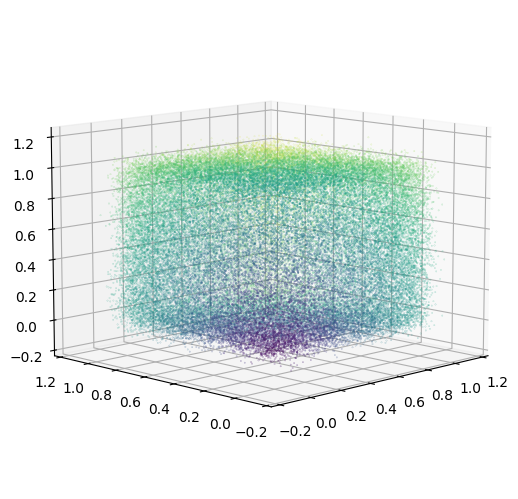
\includegraphics[width=0.9\linewidth]{python/plots/cube_points/data/cube_points}
    \end{subfigure}%
    \begin{subfigure}[b]{0.25\textwidth}
        \centering
        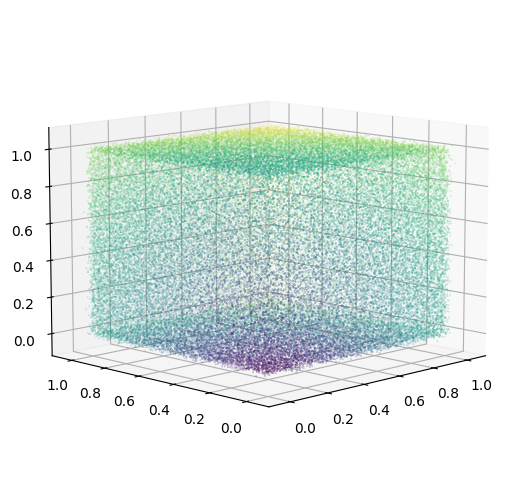
\includegraphics[width=0.9\linewidth]{python/plots/cube_points/data/noise/cube_points_noise_01}
    \end{subfigure}%
    \begin{subfigure}[b]{0.25\textwidth}
        \centering
        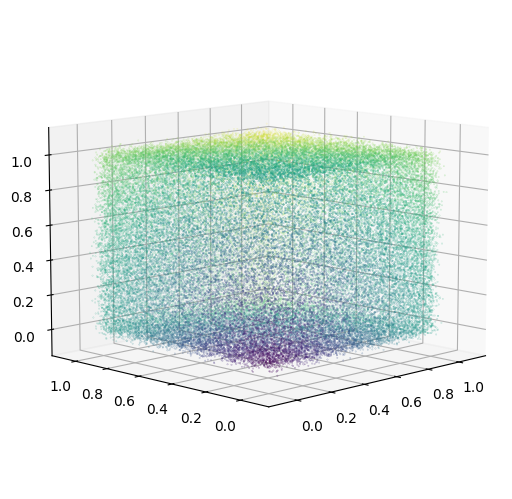
\includegraphics[width=0.9\linewidth]{python/plots/cube_points/data/noise/cube_points_noise_02}
    \end{subfigure}%
    \begin{subfigure}[b]{0.25\textwidth}
        \centering
        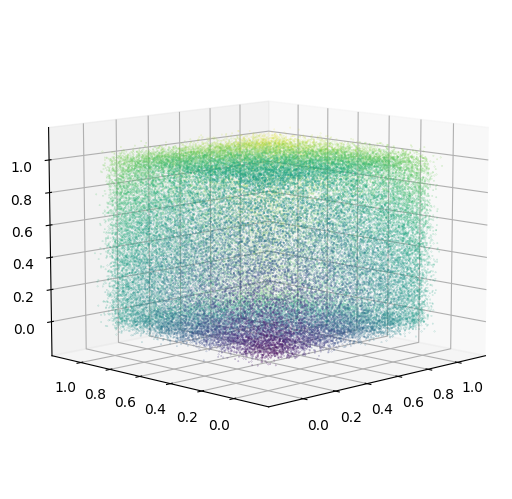
\includegraphics[width=0.9\linewidth]{python/plots/cube_points/data/noise/cube_points_noise_03}
    \end{subfigure}%

%    \vspace{0.5em}

    \begin{subfigure}[b]{0.25\textwidth}
        \centering
        
\includegraphics[width=0.9\linewidth]{python/plots/cube_points/data/cube_points_primitives}
        \caption{Noise level 0.00}
    \end{subfigure}%
    \begin{subfigure}[b]{0.25\textwidth}
        \centering
        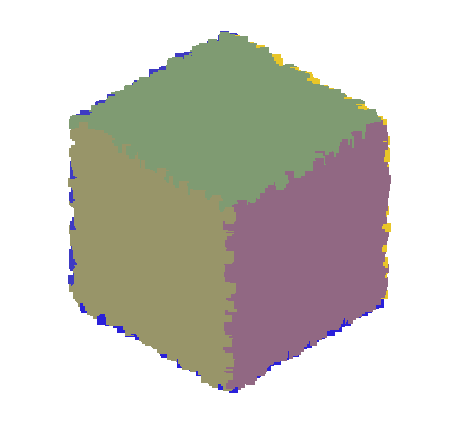
\includegraphics[width=0.9\linewidth]{python/plots/cube_points/data/noise/cube_points_noise_01_primitives}
        \caption{Noise level 0.01}
    \end{subfigure}%
    \begin{subfigure}[b]{0.25\textwidth}
        \centering
        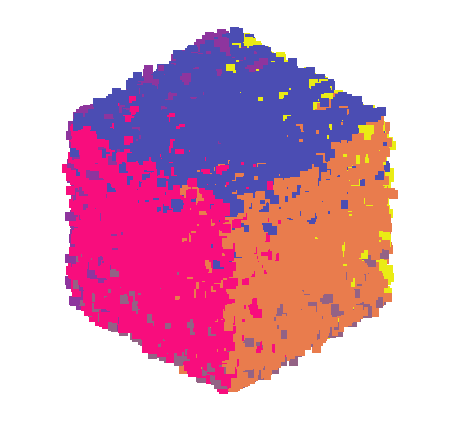
\includegraphics[width=0.9\linewidth]{python/plots/cube_points/data/noise/cube_points_noise_02_primitives}
        \caption{Noise level 0.02}
    \end{subfigure}%
    \begin{subfigure}[b]{0.25\textwidth}
        \centering
        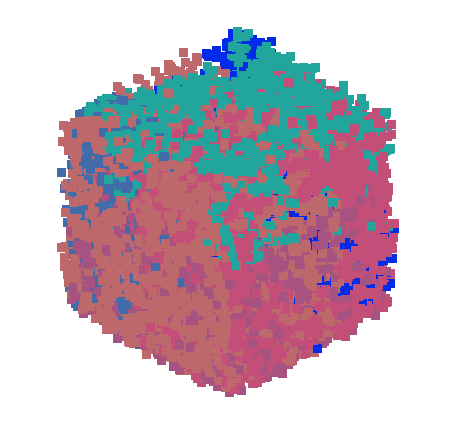
\includegraphics[width=0.9\linewidth]{python/plots/cube_points/data/noise/cube_points_noise_03_primitives}
        \caption{Noise level 0.03}
    \end{subfigure}%

    \caption{Unit cube with varying noise level}
    \label{fig:test-noise}
\end{figure}

\subsubsection{Resilience to Missing Data}

As a big problem of depth from motion techniques is the lack of depth information in areas with minimal texture,
the resilience to missing data is crucial.
In figure~\ref{fig:test-missing}, points towards the center of the cubes surfaces have been removed.
This mimics the structure of real world data from the Depth API,
as edges are often detected more accurately than surfaces,
as visible in the confidence maps of the bathroom tiles and white furniture in figure~\ref{fig:materials}.
To simulate this effect, points have been removed with an increasing probability based on the
quadratic distance to the center of the face the points belongs to.

The algorithm is able to correctly recognize the faces of the cube with a missing level up to 24.
With a missing level of 48, the algorithm still detects the planes, but doesn't assign all points to the faces.
With increasing missing level, the n parameter, which defines the minimum number of points required to fit a primitive,
is also required to be lowered.
In real world applications this would lead to more false detections, primitives being detected where there are none.

%Given a point $x$ with coordinates $(x_1, x_2, x_3)$, edge length $l$, and missing data rate $r$,
%the distance to the closest edge can be calculated as |
%
%As the cube is centered at the origin and aligned with the axis, the absolute of one coordinate will always equal $l/2$.
%By filtering out this coordinate, the point $x$ can be projected onto the plane of the cube,
%resulting in point $x'$ with coordinates $(x'_1, x'_2)$.
%
%The probability $p$ of a point being removed can then be calculated as

%\begin{equation}
%    p = \left(\frac{\sqrt{(l/2 - |x'_1|) \cdot (l/2 - |x'_2|)}}{l / 2}\right)^2 \cdot r
%\end{equation}

\begin{figure}[h!tbp]
    \centering
    % First row
    \begin{subfigure}[b]{0.25\textwidth}
        \centering
        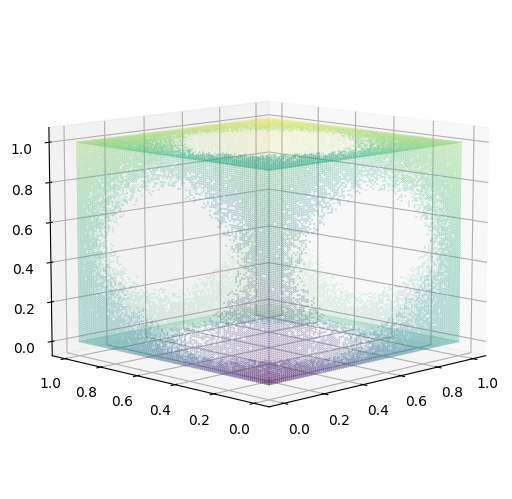
\includegraphics[width=0.9\linewidth]{python/plots/cube_points/data/missing/cube_points_missing_6_0}
    \end{subfigure}%
    \begin{subfigure}[b]{0.25\textwidth}
        \centering
        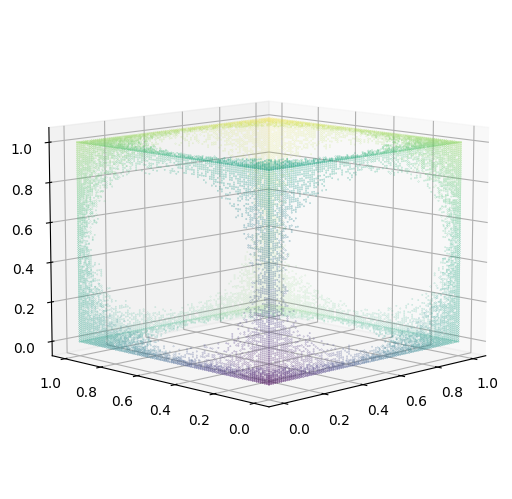
\includegraphics[width=0.9\linewidth]{python/plots/cube_points/data/missing/cube_points_missing_12}
    \end{subfigure}%
    \begin{subfigure}[b]{0.25\textwidth}
        \centering
        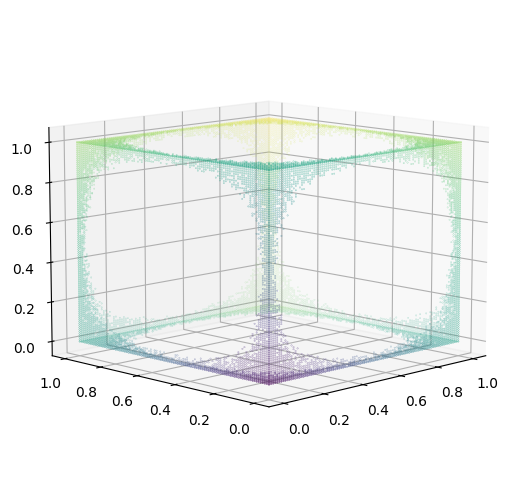
\includegraphics[width=0.9\linewidth]{python/plots/cube_points/data/missing/cube_points_missing_24}
    \end{subfigure}%
    \begin{subfigure}[b]{0.25\textwidth}
        \centering
        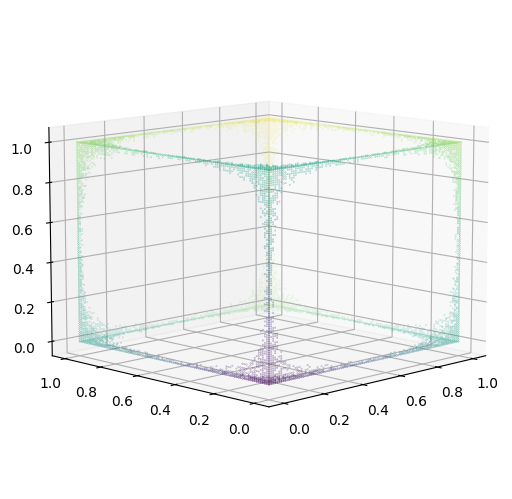
\includegraphics[width=0.9\linewidth]{python/plots/cube_points/data/missing/cube_points_missing_48}
    \end{subfigure}%

%    \vspace{0.5em}

    \begin{subfigure}[b]{0.25\textwidth}
        \centering
        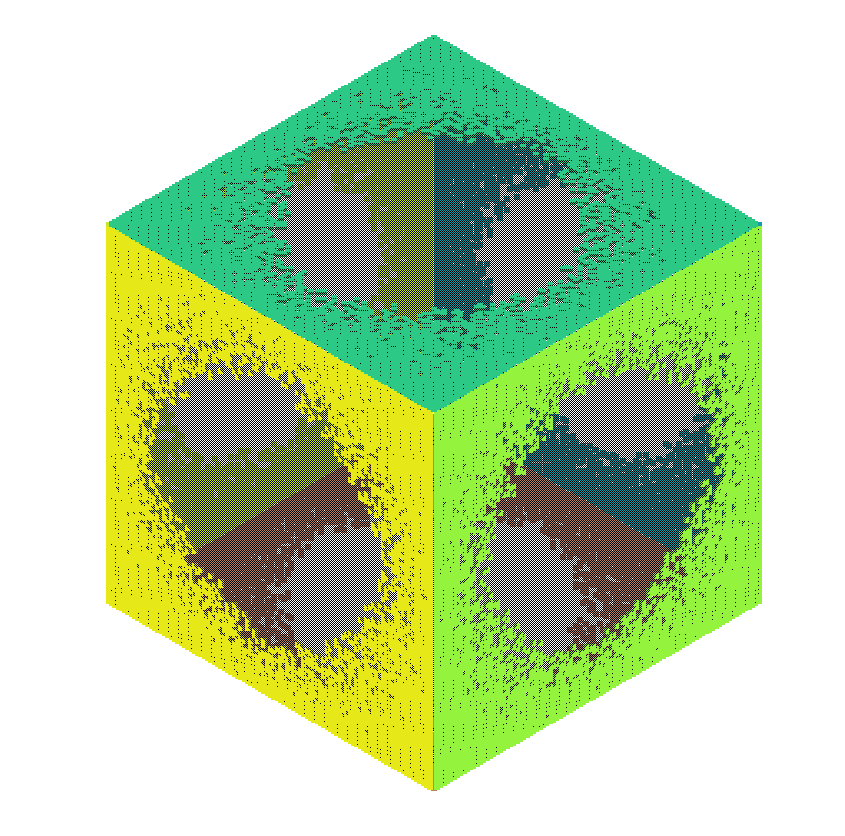
\includegraphics[width=0.9\linewidth]{python/plots/cube_points/data/missing/cube_points_missing_6_primitives}
        \caption{Missing level 6}
    \end{subfigure}%
    \begin{subfigure}[b]{0.25\textwidth}
        \centering
        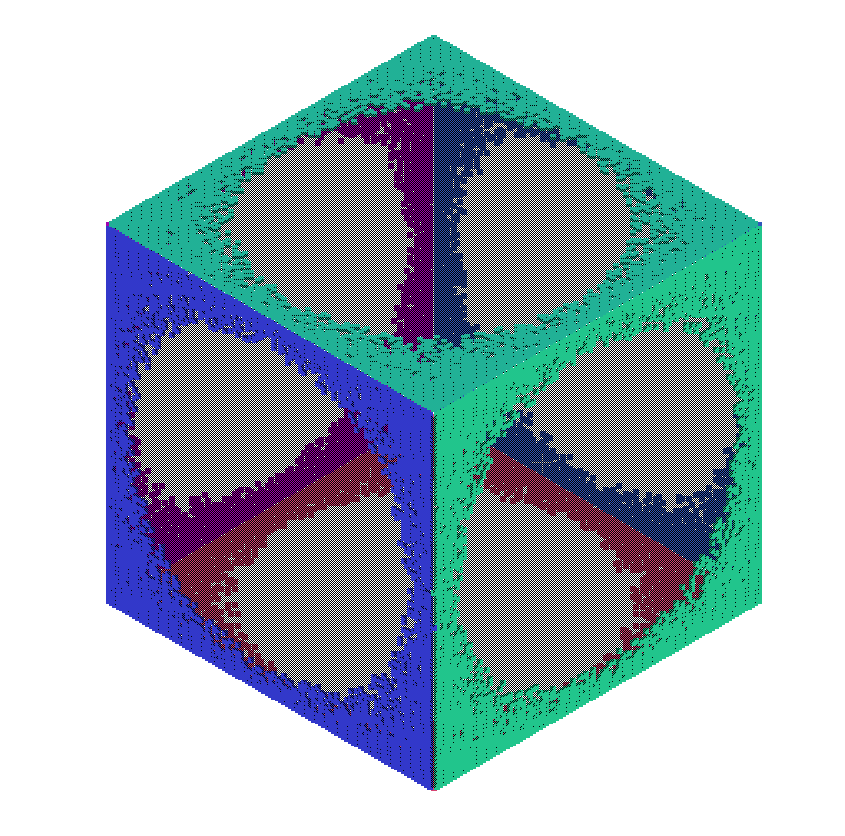
\includegraphics[width=0.9\linewidth]{python/plots/cube_points/data/missing/cube_points_missing_12_primitives}
        \caption{Missing level 12}
    \end{subfigure}%
    \begin{subfigure}[b]{0.25\textwidth}
        \centering
        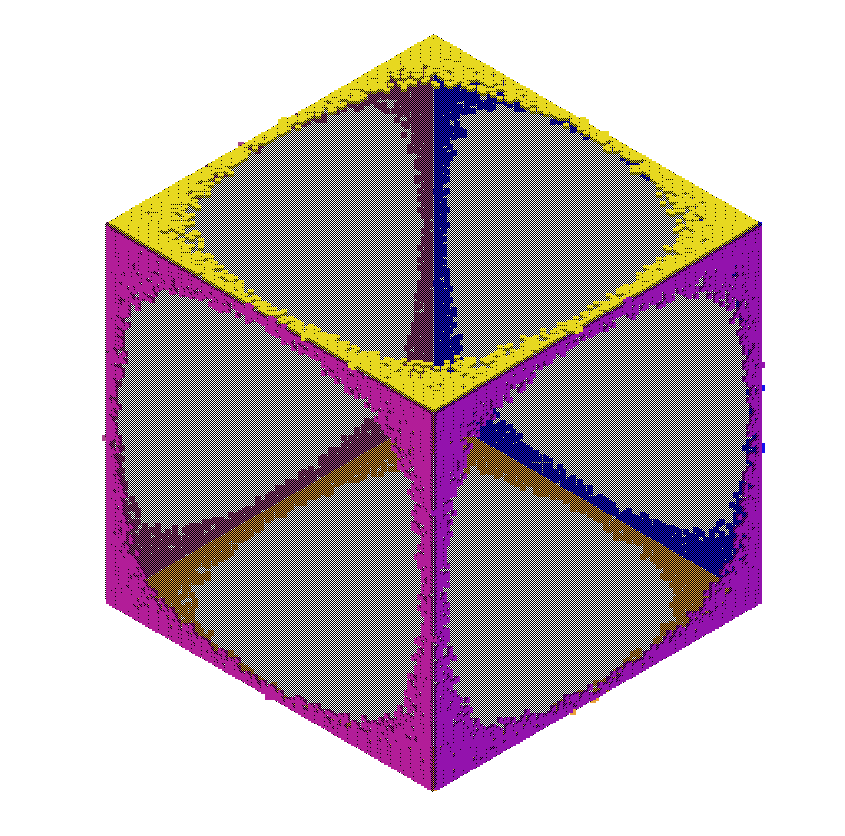
\includegraphics[width=0.9\linewidth]{python/plots/cube_points/data/missing/cube_points_missing_24_primitives}
        \caption{Missing level 24}
    \end{subfigure}%
    \begin{subfigure}[b]{0.25\textwidth}
        \centering
        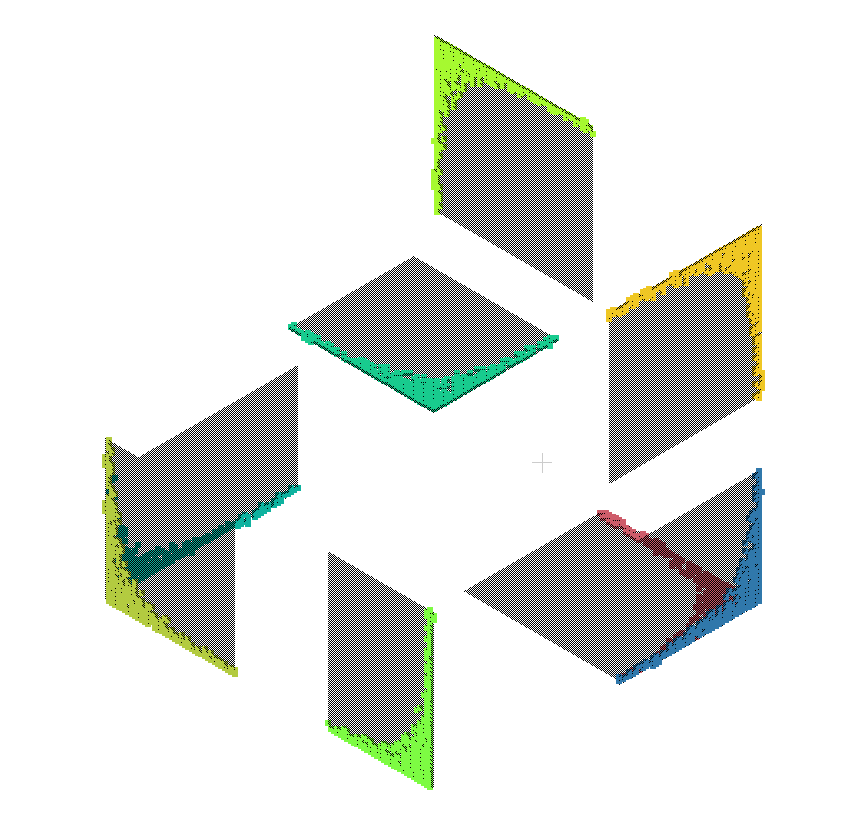
\includegraphics[width=0.9\linewidth]{python/plots/cube_points/data/missing/cube_points_missing_48_primitives}
        \caption{Missing level 48}
    \end{subfigure}%

    \caption{Unit cube with varying missing level}
    \label{fig:test-missing}
\end{figure}

\subsubsection{Resilience to Noise and Missing Data Combined}

When combining both noise and missing data, the quality of the detection is much worse.
In figure~\ref{fig:test-both}, the cube is shown with a noise level of 0.01 and varying missing levels.
With noise level 0.01 and missing level 6, the cube is still recognized correctly.
With missing level 12, more than 6 faces are being recognized, but all the points are still assigned to primitives.
This might be due to the shapes not being recognized as connected shapes,
which causes the algorithm to only fit the largest connected component of the points and will create a new parameterization
for the remaining points.
To achieve results with a missing level of 24, the epsilon parameter had to be increased to 0.015 to achieve any results at all.
As visible from the figure, the cube is not recognized correctly, with only small parts of the cube being recognized.
When increasing the noise level to 0.02, the algorithm yields no satisfactory results with any missing level, even with tweaking the parameters.

\begin{figure}[ht!]

    \centering
    % First row
    \begin{subfigure}[b]{0.25\textwidth}
        \centering
        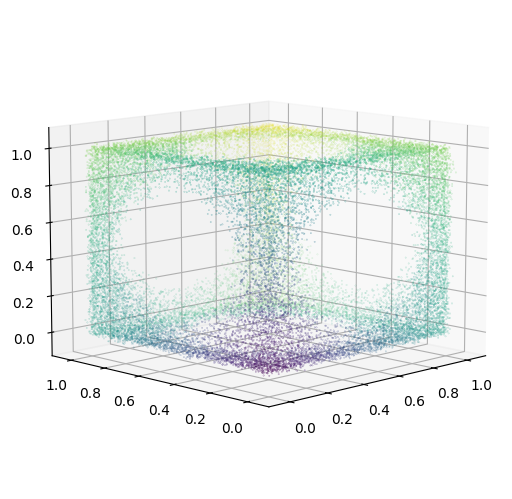
\includegraphics[width=0.9\linewidth]{python/plots/cube_points/data/matrix/cube_points_m6_n01}
    \end{subfigure}%
    \begin{subfigure}[b]{0.25\textwidth}
        \centering
        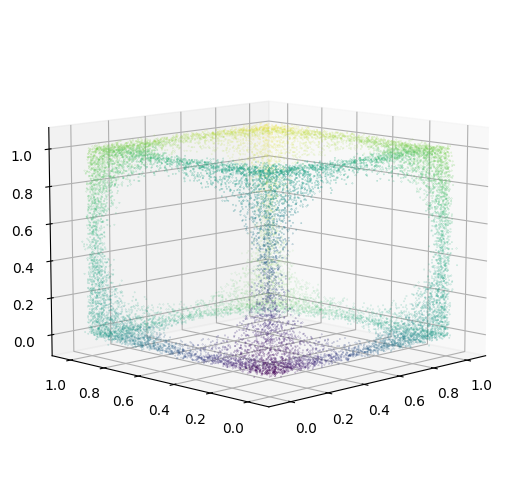
\includegraphics[width=0.9\linewidth]{python/plots/cube_points/data/matrix/cube_points_m12_n01}
    \end{subfigure}%
    \begin{subfigure}[b]{0.25\textwidth}
        \centering
        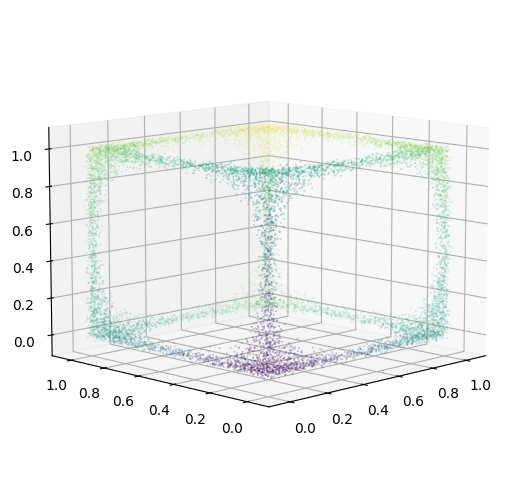
\includegraphics[width=0.9\linewidth]{python/plots/cube_points/data/matrix/cube_points_m24_n01}
    \end{subfigure}%

%    \vspace{0.5em}

    \begin{subfigure}[b]{0.25\textwidth}
        \centering
        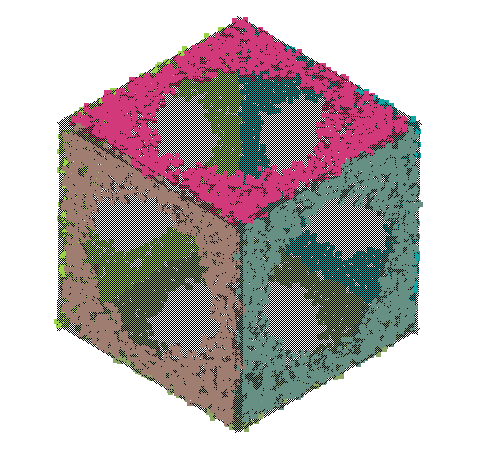
\includegraphics[width=0.9\linewidth]{python/plots/cube_points/data/matrix/cube_points_m6_n01_primitives}
        \caption{Missing level 6}
    \end{subfigure}%
    \begin{subfigure}[b]{0.25\textwidth}
        \centering
        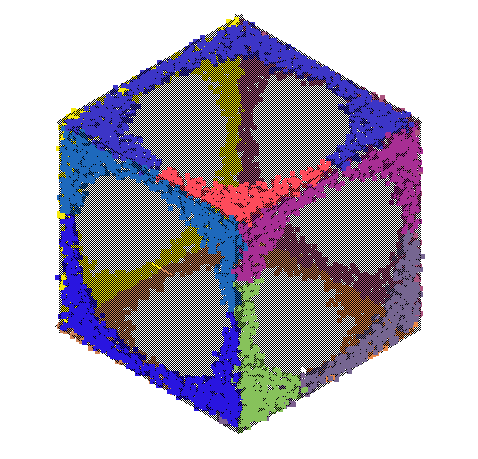
\includegraphics[width=0.9\linewidth]{python/plots/cube_points/data/matrix/cube_points_m12_n01_primitives}
        \caption{Missing level 12}
    \end{subfigure}%
    \begin{subfigure}[b]{0.25\textwidth}
        \centering
        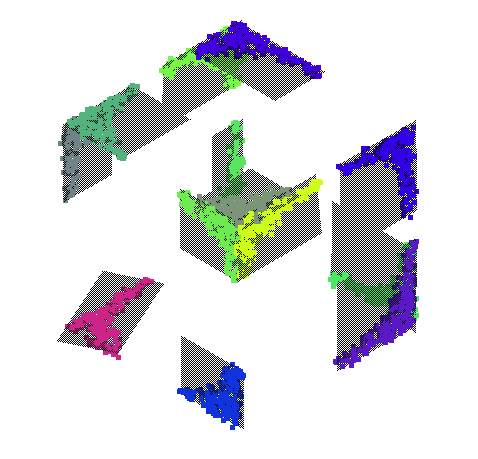
\includegraphics[width=0.9\linewidth]{python/plots/cube_points/data/matrix/cube_points_m24_n01_primitives}
        \caption{Missing level 24}
    \end{subfigure}%
    \caption{Unit cube with noise level = 0.01 and varying missing level}
    \label{fig:test-both}

\end{figure}

\subsection{Tests on Real World Data}\label{subsec:ransac-tests-on-real-world-data}

Figure~\ref{fig:real-data-ransac} show the results of the RANSAC algorithm on the dataset created with the epsilon octree,
as seen in figure~\ref{fig:octrees-compairison-epsilon}.
Note that CloudCompare uses AABBs to represent the planes, instead of the convex hull as used in the application.
In the segmented dataset, the cube is recognized correctly, with all 5 faces being recognized.
In the raw dataset, the faces of the cubes are still recognized, but the algorithm also recognizes other planes in the dataset,
some of which contain a subset of the points of the cube.
This shows a limitation of the RANSAC algorithm, which is similar to~\cite{tarsha-kurdi_hough-transform_2007} findings,
where plane primitives are constructed from points which do not belong to the same plane.
\cite{schnabel_efficient_2007} solution to this problem is using a bitmap to detect connected shapes, as mentioned in section~\ref{subsec:schnabels-efficient-ransac-algorithm}.
Only the largest connected shape in a given shape candidate is kept.
As the points that are not part of the largest connected shape are kept in the dataset, the algorithm will still consider them in the next iterations.
However, if the resulting separate primitives then do not cross the support threshold, they are filtered out.
In other words, the bitmap epsilon parameter $\beta$ can be used to adjust the resolution of the bitmap,
with higher values leading to shapes being detected as separate shapes quicker, while the minimum support threshold $n$
can be used to filter out shapes that are not supported by enough points.

\begin{figure}[htb]
    \centering

    \begin{subfigure}[b]{0.5\textwidth}
        \centering
        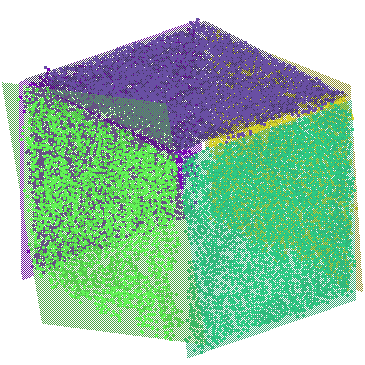
\includegraphics[width=0.7\linewidth]{images/results_cube}
        \caption{Segmented dataset, default parameters}
        \label{fig:real-data-ransac-segmented}
    \end{subfigure}%

    \vspace{0.5em}

    \begin{subfigure}[b]{0.5\textwidth}
        \centering
        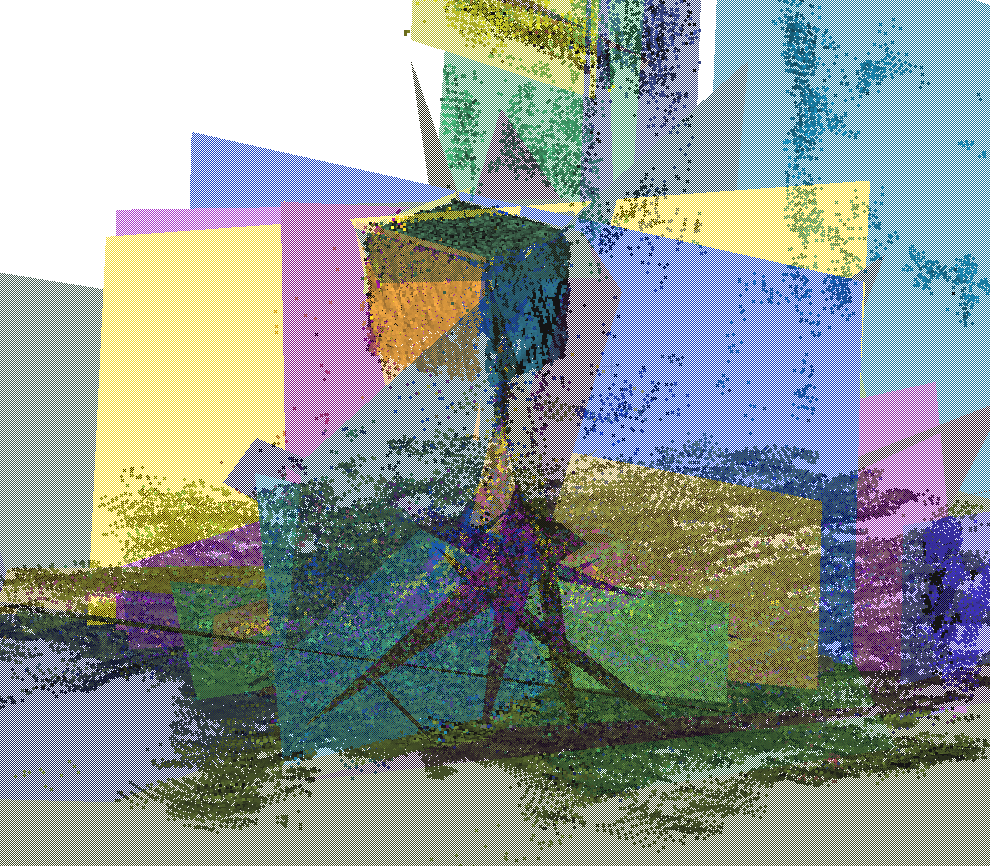
\includegraphics[width=0.7\linewidth]{images/results_all}
        \caption{Raw dataset, $n=400, \epsilon=0.024, \beta=0.047$}
    \end{subfigure}%
    \begin{subfigure}[b]{0.5\textwidth}
        \centering
        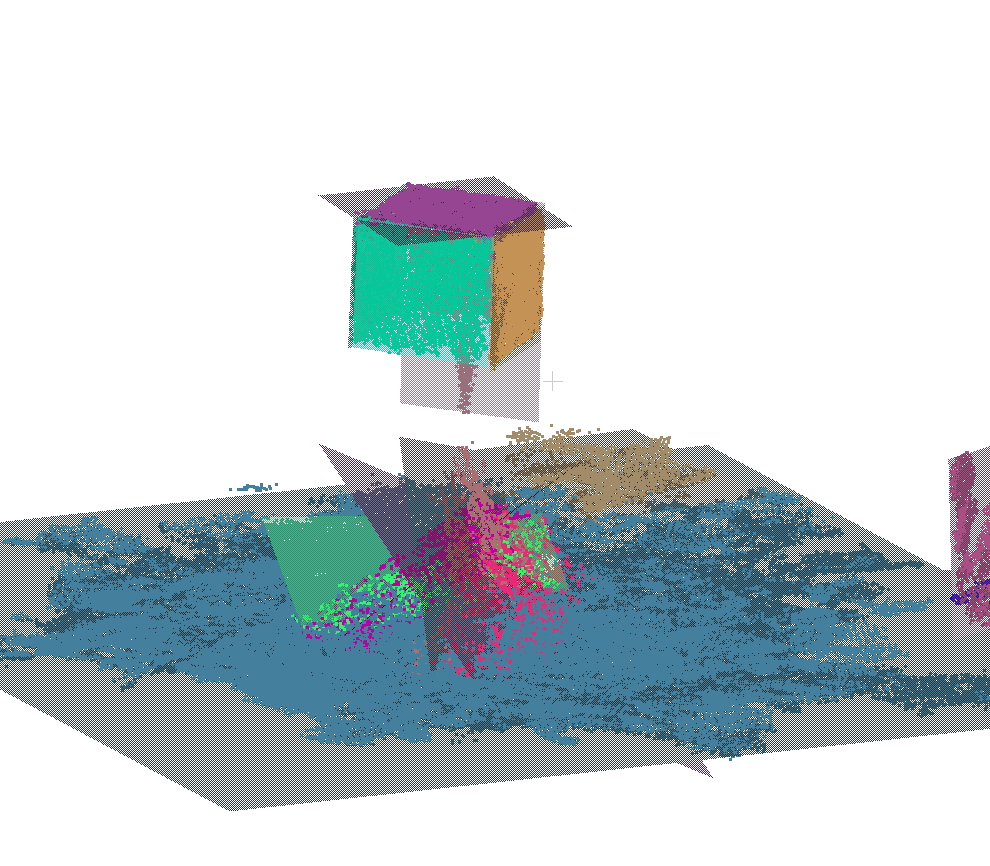
\includegraphics[width=0.7\linewidth]{images/results-all-2}
        \caption{Raw dataset, $n=400, \epsilon=0.024, \beta=0.005$}
    \end{subfigure}%
    \caption{RANSAC results on real data set collected using the epsilon octree}
    \label{fig:real-data-ransac}
\end{figure}

In the case of the dataset visible in figure~\ref{fig:real-data-ransac},
the default value of the bitmap epsilon parameter was set to $\beta=0.024$.
Ideally, the bitmap epsilon parameter would be set to the sample resolution of the dataset~\parencite{schnabel_efficient_2007}.
When raising the resolution to $\beta=0.005$, the detection results of the cube are improved,
while still detecting some artifacts that shouldn't be detected.
With these parameters, the planes in the background are also no longer detected,
as their effective sampling resolution is too low, which causes them to be detected as many separate shapes that do not cross the support threshold.
This shows that applying the algorithm to a dataset with vastly varying sampling resolutions will
lead to suboptimal results, as the parameters need to be set for the whole dataset.
This is problematic for the use case in combination with the depth from motion algorithm, as the Raw Depth API
will have low confidence in areas with low texture, which will cause lower sampling rates, or completely missing data,
which will in turn lead to connected shapes not being present and being filtered out.
It is therefore difficult to find a parameterization for the algorithm that fits both highly textured and low-textured objects.


\section{Application Performance}\label{sec:application-performance}

This section will evaluate the combined performance of the application, first on the test cube, then on a full room scan.

\subsection{Test Cube}\label{subsec:application-performance-test-cube}
Figure~\ref{fig:cube-results} shows the results of a scan of the test cube under the same procedure as in section~\ref{sec:point-clouds} with varying sample resolution $s$.
Note that the point cloud is not segmented in the application, thus other planes (namely the floor) are also detected in the background.
The parameters used aside from $s$ will be discussed after describing the results.

With an epsilon octree resolution of $s=0.015$, one of the faces is merged with points from the stand the cube is placed on.
Starting with a resolution of $s=0.010$, all the 5 faces are recognized correctly and
the convex hull algorithm correctly creates a matching polygon for each face, with small gaps between the faces.
Increasing the resolution further to $s=0.005$ improves the accuracy of the edges of the planes slightly.
While there are no longer gaps between the faces, some amount of clipping is now visible in the polygons.
%With the selected parameters, a total of 250.000 points were collected and processed by the RANSAC algorithm in about 20 seconds.

\begin{figure}[h!tbp]
    \centering

    \begin{subfigure}[b]{\textwidth}
        \centering
        \includegraphics[width=0.3\linewidth]{images/cube_015_1}
        \includegraphics[width=0.3\linewidth]{images/cube_015_2}
        \includegraphics[width=0.3\linewidth]{images/cube_015_3}
        \caption{$s=0.015, n\approx60.000$}
        \label{fig:cube-results-0015}
    \end{subfigure}%

    \vspace{0.5em}

    \begin{subfigure}[b]{\textwidth}
        \centering
        \includegraphics[width=0.3\linewidth]{images/cube_010_1}
        \includegraphics[width=0.3\linewidth]{images/cube_010_2}
        \includegraphics[width=0.3\linewidth]{images/cube_010_3}
        \caption{$s=0.010, n\approx125.000$}
    \end{subfigure}%

    \vspace{0.5em}

    \begin{subfigure}[b]{\textwidth}
        \centering
        \includegraphics[width=0.3\linewidth]{images/cube_005_1}
        \includegraphics[width=0.3\linewidth]{images/cube_005_2}
        \includegraphics[width=0.3\linewidth]{images/cube_005_3}
        \caption{$s=0.005, n\approx250.000$}
    \end{subfigure}%

    \caption{Detection results of the test cube using the mobile application}
    \label{fig:cube-results}
\end{figure}

Using a trial-and-error approach, the parameters of the RANSAC algorithm were adjusted to achieve the best trade-off between
performance, the amount of detected planes and noise.
The final parameters used are:
\begin{itemize}
    \item $0.010\geq s \geq 0.005$ -- The resolution of the epsilon octree.
    Higher resolutions than 0.005 lead to a significantly higher amount of points and thus worse runtime performance without noticeable improvements in the detection results,
    while lower resolutions than 0.010 lead to visibly worse results, with outliers having a bigger impact on the detection results, as visible in figure~\ref{fig:cube-results-0015}.
    \item $n=\left(\frac{1}{s}\right)^2\cdot0.15^2=900$ -- The minimum number of points required to fit a primitive.
    Equal to the amount of points on a $15cm^2$ plane, if uniformly sampled with $s$.
    Realistically, this number will be lower, as the points are scattered across the normal of the plane.
    However, the epsilon octree also has a lower actual resolution than $s$, as discussed in section~\ref{subsec:quantization-octree-vs.-epsilon-octree},
    which should cancel out the effect.
    The calculation is only a rough estimate and proved to show good results.
    \item $\epsilon=0.022$ -- The epsilon parameter of the RANSAC algorithm.
    Lower values lead to planes being detected as multiple planes along the planes normal.
    This parameter varies depending on noise of the data.
    Two standard deviations contain 95.5 percent of all data, which is used as a starting point.
    As the epsilon octree showed a standard deviation of 0.011, a value of 0.022 is chosen and shows good results.
    \item $\beta=1.5s$ -- The epsilon parameter of the bitmap.
    As discussed in~\ref{subsec:ransac-tests-on-real-world-data}, settings this parameter is a trade of between detecting shapes that have missing data and filtering out shapes that are not connected in reality.
    $1.5s$ is a rather strict value that filters out most shapes with gaps in their data due to missing texture, however it greatly reduces the amount of artifacts.
\end{itemize}
Other parameters are kept at their default values.
As all parameters except $\epsilon$ are relative to $s$,
it should be easy to adapt the parameters to different devices that might offer depth maps with other accuracies -
only the resolution of the epsilon octree has to be adjusted.
As for $\epsilon$, the parameter needs to be adjusted based on the noise level of the data, which might vary based on the device and the lighting conditions.


As for runtime performance, the device remains responsive with $\epsilon\geq0.005$, however it heats
up quickly and the application experiences a significant slowdown after a few scans.
This is due to both the creation of the point cloud using the epsilon octree and the RANSAC algorithm being
very computationally expensive.

\subsection{Full Room Scan}\label{subsec:application-performance-full-room}

For a full room scan, the device is moved around the room in a similar fashion as described in section~\ref{sec:point-clouds}.
The room is scanned from multiple angles to capture all surfaces.
In total, about 500.000 points are collected and processed by the RANSAC algorithm.
The processing time of the RANSAC algorithm is about two minutes, which is significantly longer than for the test cube.
Figure~\ref{fig:full-room-scan-results} shows the results of a full room scan.
In general, the results can be described as mixed.
The walls and floor are mostly recognized correctly, while some parts of them are missing.
The decent results on the wall can be explained by the lighting conditions, as the walls are lit from a window at an angle,
which creates shadows that increase the texture of the wall.
In contrast, white furniture is almost not recognized at all, as the low texture of the material leads
to missing data.
When it comes to smaller objets, the algorithm struggles to correctly recognize them, as the data is too noisy,
as is visible from the capture of the desk, where artifacts are visible in the detection results.

In conclusion, the application is able to detect primitives in a full room scan,
however the results are not sufficient to build a full mesh of the room.
The processing time of the RANSAC algorithm is also too high to be used in most real-time applications.

\begin{figure}[h!tbp]
    \centering
    \includegraphics[width=0.9\linewidth]{images/full_room_3}
    \includegraphics[width=0.9\linewidth]{images/full_room_2}
    \includegraphics[width=0.9\linewidth]{images/full_room_1}
    \caption{Detection results of a full room scan using the mobile application. $s=0.010, n\approx500.000$}
    \label{fig:full-room-scan-results}
\end{figure}

